\documentclass[11pt,a4paper]{article}

% --- Packages ---
\usepackage[a4paper,margin=1in]{geometry}
\usepackage{graphicx}
\usepackage{lmodern}
\usepackage[T1]{fontenc}
\usepackage[utf8]{inputenc}
\usepackage{microtype}
\usepackage{parskip}
\usepackage{xcolor}
\usepackage{hyperref}
\usepackage{url}
\usepackage{amsmath}


% --- Colors & Links ---
\definecolor{facultyblue}{HTML}{0055A4} % adjust if you prefer a different blue
\hypersetup{
  colorlinks=true,
  linkcolor=facultyblue,
  urlcolor=facultyblue
}

% --- Metadata Macros (edit here) ---
\newcommand{\InstructorNames}{Marra Giuseppe \& Meert Wannes}
\newcommand{\CourseName}{Machine Learning: Project}
\newcommand{\CourseCode}{H0T25a}
\newcommand{\StudentName}{Benjamin Droogmans}
\newcommand{\StudentID}{r0890563}
\newcommand{\AcademicYear}{2024--2025}
\newcommand{\FacultyLogo}{./figures/logo-firw-eng-tekst-blauw.png}

% Optional PDF metadata
\hypersetup{
  pdftitle={\CourseName\ (\CourseCode) -- Project Report},
  pdfauthor={\StudentName\ (\StudentID)},
  pdfsubject={\CourseName\ Project},
  pdfkeywords={Machine Learning, Project, \CourseCode}
}

\begin{document}

% --- Front page ---
\begin{titlepage}
\thispagestyle{empty}

% Top accent bar
{\color{facultyblue}\rule{\textwidth}{3pt}}

\vspace{1.5em}

% Logo (top-right)
\begin{flushright}
  \includegraphics[height=2.2cm]{\FacultyLogo}
\end{flushright}

% Title block
\vspace*{1em}
{\huge\bfseries \CourseName\par}
\vspace{0.15em}
{\Large\bfseries (\CourseCode)\par}

\vspace{2.2em}

% Info block
\begingroup
\setlength{\tabcolsep}{0pt}
\renewcommand{\arraystretch}{1.35}
\begin{tabular}{@{}p{3.6cm} l}
\textbf{Instructors:}    & \InstructorNames \\
\textbf{Student:}        & \StudentName\ (\StudentID) \\
\textbf{Academic year:}  & \AcademicYear \\
\end{tabular}
\endgroup

\vfill

% Bottom accent bar
{\color{facultyblue}\rule{\textwidth}{1.5pt}}

\end{titlepage}



% --- (Optional) structure for the rest of the report ---
\pagenumbering{roman}
\tableofcontents
\clearpage
\pagenumbering{arabic}

% Example content include (remove if you don't want placeholders)
\section{Introduction}
Machine learning is one of the most active and innovative research fields today. Outside of the big theoretic advancements, a lot of practical applications find their way into the world. In practical settings two aspects often arise. Often the state space is enourmous, so that that an approximate solution is the only option. This gives rise to Deep learning where Neural Networks (NN) are used to approximate complicated state-action functions. In the real world we are often not alone. This gives rise to the second common aspect to Machine Learning problems. Entire research fields exist to study what happens when multiple actors want to achieve something simultaneously. Games are often used in research for both deep learning and agent interactions. Games are useful in this setting, because it is easy to control the environment and understand the results. They do have the power to capture delicate interactions and because of combinatorial explosion they can become quite complex. 

Task 1 is an overview of the works which are the base of our experiments. In our work we study the interaction between the fields which have studied agent interactions in task 2. Then we train a single agent to learn a complex game using deep learning in task 3. 


\section{Task 1: literature Study}

Three papers were especially influential for this work. Apart from this there is a lot of other material which was important, they are 

\paragraph{Bloembergen et al. (2015).}  
The survey on \emph{Evolutionary Dynamics of Multi-Agent Learning}
\cite{bloembergen2015evolutionary} guided \textbf{Task 2 (Matrix Games)}. It
connected game-theoretic concepts such as Nash equilibria and Pareto
efficiency with learning dynamics, and introduced replicator equations as a
tool to analyze how strategies evolve—directly shaping the analytical part of
the assignment.

\paragraph{Machado et al. (2018).}  
The study revisiting the Arcade Learning Environment \cite{machado2018revisiting}
influenced \textbf{Task 3 (Single Archer RL)} by emphasizing robust evaluation
protocols. Principles such as sticky actions, train-test seed separation, and
multi-seed evaluation inspired how experiments were designed and assessed.

\paragraph{Arulkumaran et al. (2017).}  
The brief survey on deep reinforcement learning \cite{arulkumaran2017deep}
helped frame the \textbf{algorithmic choices in Task 3}. It clarified the tradeoffs
between DQN and PPO, and highlighted common extensions, motivating the
incremental improvement path used here.

\paragraph{Summary.}  
Together, these works provided theoretical grounding for matrix games,
methodological rigor for evaluation, and practical guidance for algorithm
design.

\section{Task 2: Matrix Games}

Matrix games provide canonical testbeds for studying the interaction between learning algorithms and game-theoretic concepts in multi-agent systems. They are simple, fully specified by payoff matrices, and capture key tradeoffs that appear in more complex environments. In this work, four well-established benchmark games are considered: the \emph{Stag Hunt} (a coordination game), the \emph{Subsidy Game} (a coordination game with asymmetric incentives), \emph{Matching Pennies} (a zero-sum game), and the \emph{Prisoner’s Dilemma} (a social dilemma). Each of these games highlights distinct strategic patterns such as risk-dominance, dominance by defection, or the absence of pure strategy equilibria. The Nash equilibria and Pareto optimal outcomes listed below give insight into the structure of the games. Then agents learn to play these games using various learning algorithms to give insight into how learning agents behave in different strategic settings. Finally the replicator dynamicss of the algorithms are plotted to see if the theoretical predictions match the empirical results.

\begin{figure}[h]
    \centering
    \scalebox{0.85}{ % adjust scaling factor as needed
    \begin{tabular}{c c c c}
    % Stag Hunt
    \begin{tabular}{c|c c}
        & S & H \\
        \hline
        S & (1,1) & (0,2/3) \\
        H & (2/3,0) & (2/3,2/3) \\
    \end{tabular}
    &
    % Subsidy Game
    \begin{tabular}{c|c c}
        & S1 & S2 \\
        \hline
        S1 & (12,12) & (0,11) \\
        S2 & (0,11) & (10,10) \\
    \end{tabular}
    &
    % Matching Pennies
    \begin{tabular}{c|c c}
        & H & T \\
        \hline
        H & (1,-1) & (-1,1) \\
        T & (-1,1) & (1,-1) \\
    \end{tabular}
    &
    % Prisoner's Dilemma
    \begin{tabular}{c|c c}
        & C & D \\
        \hline
        C & (3,3) & (0,5) \\
        D & (5,0) & (1,1) \\
    \end{tabular}
    \end{tabular}
    }
    \caption{Payoff matrices of the four benchmark games: Stag Hunt, Subsidy Game, Matching Pennies, and Prisoner’s Dilemma.}
\end{figure}



\subsection{Nash Equilibria and Pareto Optimal Outcomes}

The four benchmark games are analyzed in terms of their Nash equilibria and Pareto optimal outcomes, based on the payoff matrices defined above.

\paragraph{Stag Hunt.}  
The Stag Hunt is a coordination game. Two pure strategy Nash equilibria exist: $(S,S)$ and $(H,H)$. In addition, there is a mixed equilibrium where each player hunts stag with probability $\tfrac{2}{3}$ and hare with probability $\tfrac{1}{3}$. The unique Pareto optimal outcome is $(S,S)$, which strictly improves upon all other outcomes for both players.

\paragraph{Subsidy Game.}  
The Subsidy Game is also a coordination game. Here, $(S_{1},S_{1})$ is the unique Nash equilibrium, since $S_{1}$ strictly dominates $S_{2}$ for the second player. The only Pareto optimal outcome is likewise $(S_{1},S_{1})$, as it yields the highest joint payoff.

\paragraph{Matching Pennies.}  
Matching Pennies is a constant-sum (zero-sum) game. No pure strategy Nash equilibrium exists. The unique equilibrium is in mixed strategies, where both players play heads and tails with equal probability $0.5$. In constant-sum games, no outcome strictly improves both players simultaneously. Hence, all four action profiles are Pareto optimal.

\paragraph{Prisoner’s Dilemma.}  
The Prisoner’s Dilemma is a social dilemma. The unique Nash equilibrium is $(D,D)$, since defection strictly dominates cooperation for both players. However, $(D,D)$ is Pareto dominated by $(C,C)$. The Pareto frontier consists of $(C,C)$, $(C,D)$, and $(D,C)$.


Implement yourself (a) $\epsilon$-greedy Q-learning, (b) Boltzmann Q-learning, and (c) Lenient Boltzmann Q-
learning [2]. Plot multiple empirical (time-averaged) learning trajectories. Thus, show how the policy
changes over multiple iterations of the learning step (see figure 1e for an example). Explain the behav-
ior and the differences between algorithms. Investigate and report on whether the learning algorithms
converge to a Nash equilibrium and/or a Pareto optimal state (or why not). [5/8 points]

\subsection{Learning Algorithms and Empirical Trajectories}
Three learning algorithms are implemented to study their behavior in the benchmark games. (INSERT REFERENCE TO RL BOOK AND PAPER). The algorithms and their characteristic update rule are: 

(a) $\epsilon$-greedy Q-learning, 

(b) Boltzmann Q-learning, and 

(c) Lenient Boltzmann Q-learning. 

MERGE THIS SECTION WITH DERIVATION OF THEM IN NOTEBOOK

$\epsilon$-greedy Q-learning is a simple form of Q-learning that chooses actions based on an $\epsilon$-greedy policy, balancing exploration and exploitation. Boltzmann Q-learning selects actions according to a softmax distribution over Q-values, allowing for more nuanced exploration. Lenient Boltzmann Q-learning extends this by incorporating leniency, which helps agents to be more forgiving of suboptimal actions during the learning process. (INSERT REFERENCE TO PAPER and RL BOOK).


Empirical learning trajectories show how the policies of agents evolve over time in each game. The trajectories are plotted in a simplex representation, where each vertex corresponds to a pure strategy, and points within the simplex represent mixed strategies. The temporal evolution is visualized as a color gradient, the change being proportional to the logarithm of the amount of iterations.

\paragraph{Stag Hunt.}

Empirical learning trajectories for the Stag Hunt game are shown in below. The $\epsilon$-greedy Q-learning algorithm quickly learns to coordinate, but because of the random deviations, more likely goes for the risk-averse equilibrium. Not a lot of lines are drawn, which indicates that if the agent starts in a dominated strategy, it will quickly learn to choose the more safe option. Boltzmann Q-learning seems to behave more exploratory, lingering around the mixed strategies longer. This is likely due to the softmax action selection, which allows for more exploration of suboptimal actions. The Boltzmann Q-learning algorithm also plays the more safe coordinated strategy and fails to figure out the risk-dominant strategy. Lenient Boltzmann Q-learning, on the other hand, shows a different pattern. The leniency allows agents to explore more and eventually converge to the Pareto optimal outcome $(S,S)$. The trajectories indicate that agents are more willing to try out the riskier strategy. Again the agents fail to cooperate to hunt stag. This is surprising, as the leniency should help them to explore more and find the optimal strategy. However, it seems that the leniency is not sufficient to overcome the risk associated with hunting stag when the other player is not cooperating.

\begin{figure}[h]
    \centering
    \begin{minipage}{0.32\textwidth}
        \centering
        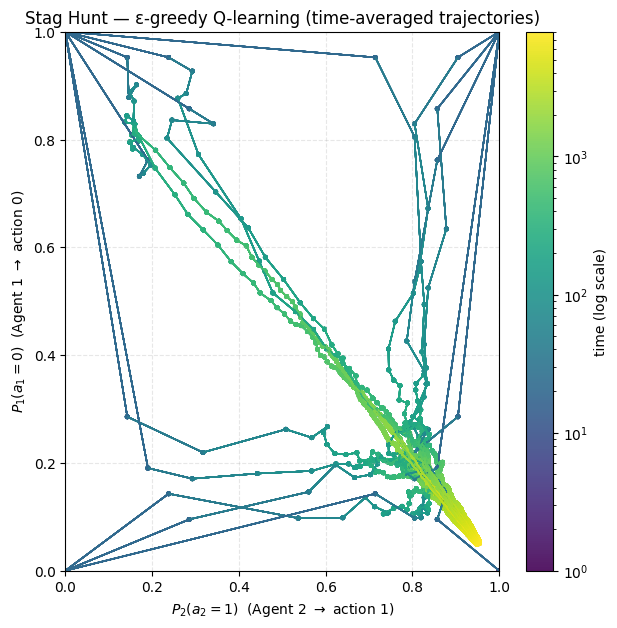
\includegraphics[width=\linewidth]{figures/task-2/learning/stag_hunt_egreedy.png}
        \caption*{(a) $\epsilon$-greedy Q-learning}
    \end{minipage}
    \hfill
    \begin{minipage}{0.32\textwidth}
        \centering
        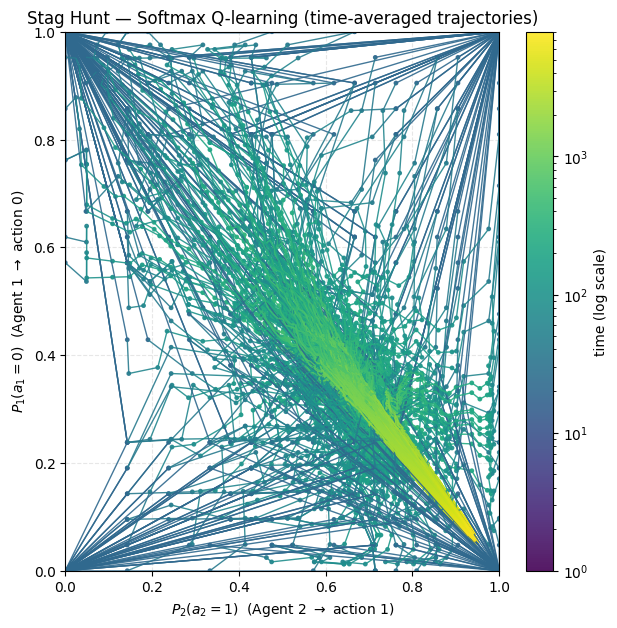
\includegraphics[width=\linewidth]{figures/task-2/learning/stag_hunt_boltz.png}
        \caption*{(b) Boltzmann Q-learning}
    \end{minipage}
    \hfill
    \begin{minipage}{0.32\textwidth}
        \centering
        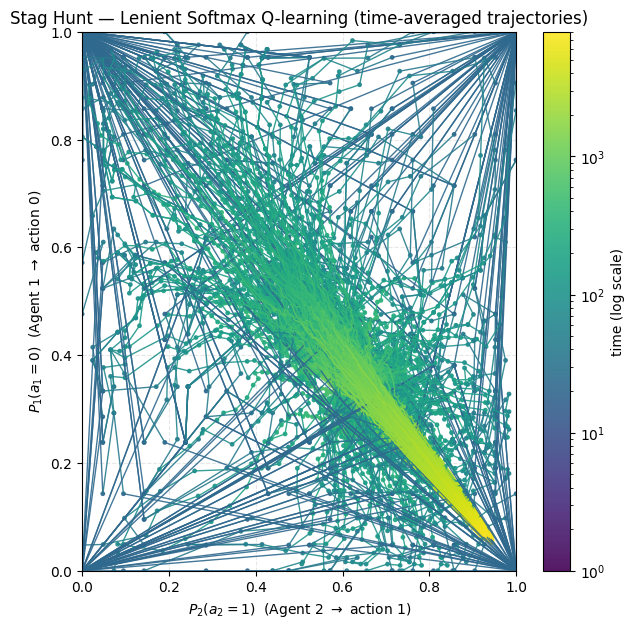
\includegraphics[width=\linewidth]{figures/task-2/learning/stag_hunt_lenient.png}
        \caption*{(c) Lenient Boltzmann Q-learning}
    \end{minipage}
    \caption{Empirical learning trajectories for the Stag Hunt game using (a) $\epsilon$-greedy Q-learning, (b) Boltzmann Q-learning, and (c) Lenient Boltzmann Q-learning.}
\end{figure}


\paragraph{Subsidy Game.}


Empirical learning trajectories for the Subsidy Game are shown below. For $\epsilon$-greedy Q-learning, agents rapidly converge to the dominant equilibrium $(S_1, S_1)$, as the incentives strongly favor this outcome. The trajectories are short, indicating fast convergence. Boltzmann Q-learning also converges to $(S_1, S_1)$, it does it so fast that the learning trajectories only show for when it learns the suboptimal policy. learing $(S_1, S_1)$ is just so quick. . Lenient Boltzmann Q-learning exhibits similar behavior, but the added leniency can result in slightly longer exploration before convergence, as agents are more tolerant of early mistakes.

\begin{figure}[h]
    \centering
    \begin{minipage}{0.32\textwidth}
        \centering
        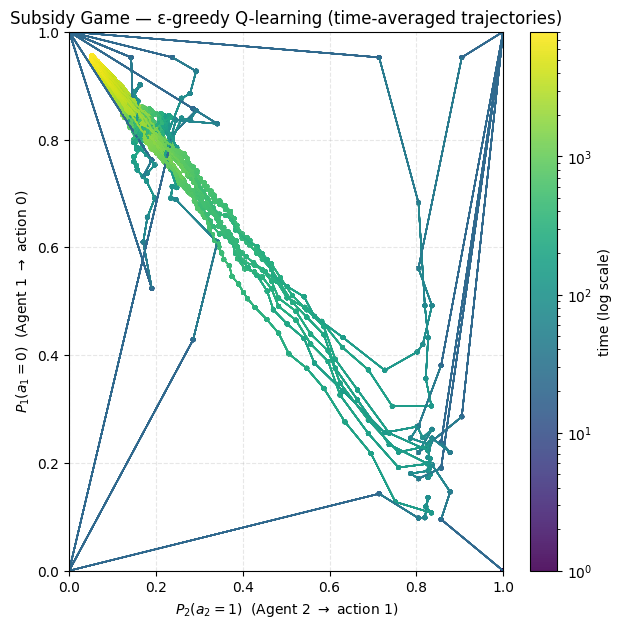
\includegraphics[width=\linewidth]{figures/task-2/learning/sg_egreedy.png}
        \caption*{(a) $\epsilon$-greedy Q-learning}
    \end{minipage}
    \hfill
    \begin{minipage}{0.32\textwidth}
        \centering
        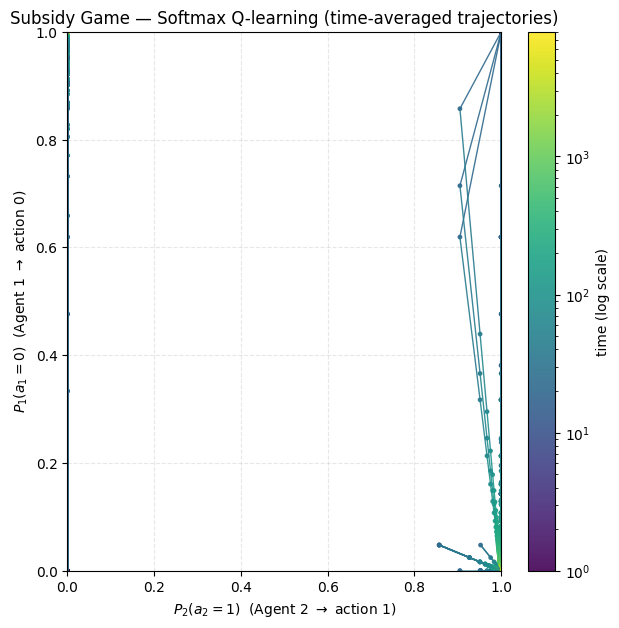
\includegraphics[width=\linewidth]{figures/task-2/learning/sg_boltz.png}
        \caption*{(b) Boltzmann Q-learning}
    \end{minipage}
    \hfill
    \begin{minipage}{0.32\textwidth}
        \centering
        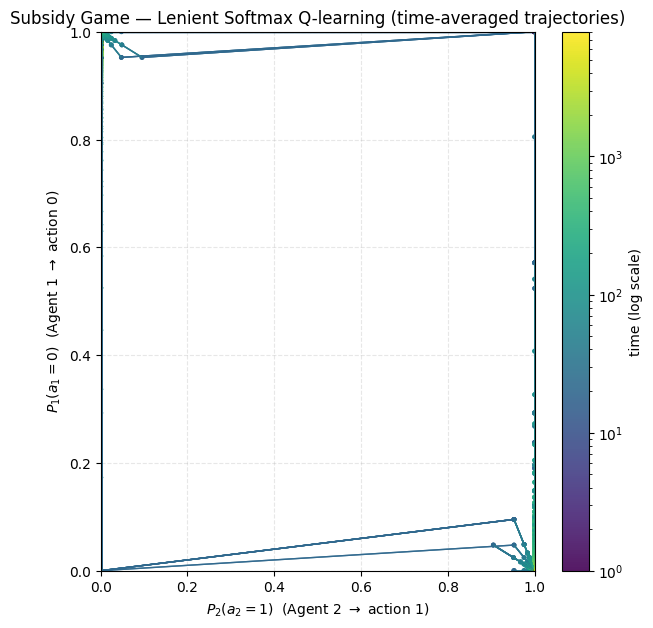
\includegraphics[width=\linewidth]{figures/task-2/learning/sg_lenient.png}
        \caption*{(c) Lenient Boltzmann Q-learning}
    \end{minipage}
    \caption{Empirical learning trajectories for the Subsidy Game using (a) $\epsilon$-greedy Q-learning, (b) Boltzmann Q-learning, and (c) Lenient Boltzmann Q-learning.}
\end{figure}


\paragraph{Matching Pennies.}
Empirical learning trajectories for Matching Pennies are shown below. The $\epsilon$-greedy Q-learning algorithm actually learns the mixed Nash equilibrium quite fast. Because of the decreasing exploration rate, the agent settles around the equilibrium. Boltzmann Q-learning also converges to the mixed strategy equilibrium, but the trajectories show more exploration around the equilibrium point, likely due to the softmax action selection. Lenient Boltzmann Q-learning exhibits similar behavior, with agents exploring more before settling into the mixed strategy equilibrium. The leniency allows for more exploration of suboptimal actions, but ultimately, agents converge to the Nash equilibrium.

\begin{figure}[h]
    \centering
    \begin{minipage}{0.32\textwidth}
        \centering
        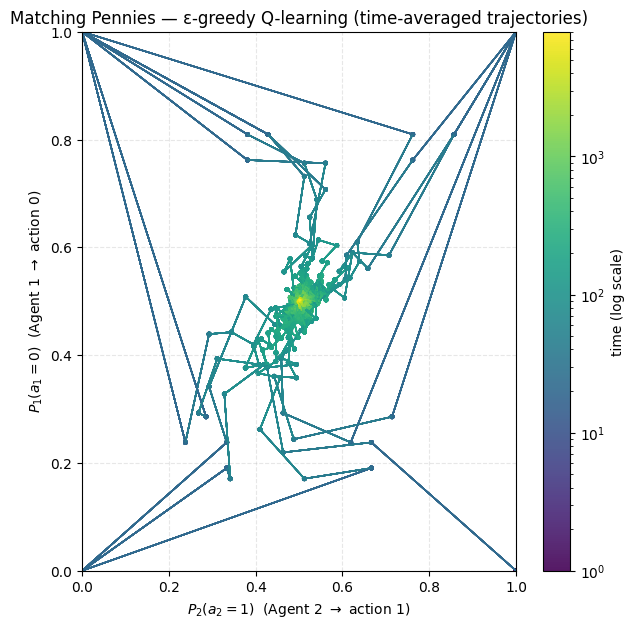
\includegraphics[width=\linewidth]{figures/task-2/learning/mp_egreedy.png}
        \caption*{(a) $\epsilon$-greedy Q-learning}
    \end{minipage}
    \hfill
    \begin{minipage}{0.32\textwidth}
        \centering
        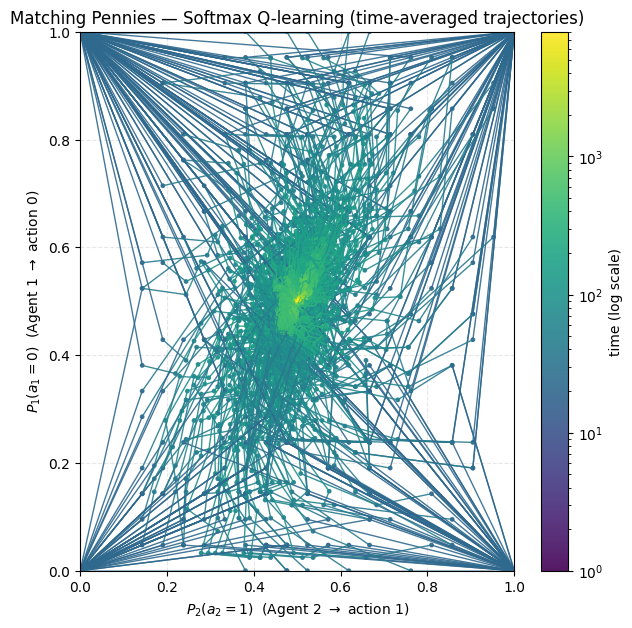
\includegraphics[width=\linewidth]{figures/task-2/learning/mp_boltz.png}
        \caption*{(b) Boltzmann Q-learning}
    \end{minipage}
    \hfill
    \begin{minipage}{0.32\textwidth}
        \centering
        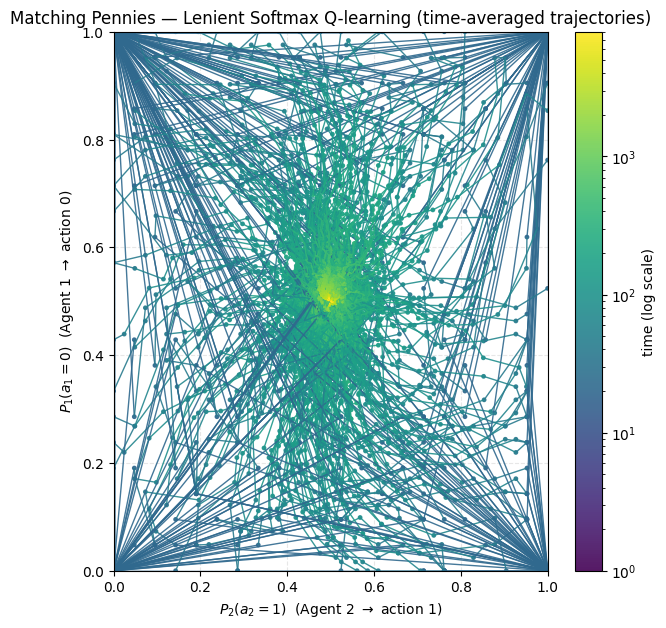
\includegraphics[width=\linewidth]{figures/task-2/learning/mp_lenient.png}
        \caption*{(c) Lenient Boltzmann Q-learning}
    \end{minipage}
    \caption{Empirical learning trajectories for Matching Pennies using (a) $\epsilon$-greedy Q-learning, (b) Boltzmann Q-learning, and (c) Lenient Boltzmann Q-learning.}
\end{figure}


\paragraph{Prisoner’s Dilemma.}
Empirical learning trajectories for the Prisoner’s Dilemma are shown below. The $\epsilon$-greedy Q-learning algorithm quickly converges to the dominant strategy $(D,D)$, as defection strictly dominates cooperation. The trajectories are short, indicating fast convergence. Boltzmann Q-learning also converges to $(D,D)$, with trajectories showing some exploration of cooperative strategies before settling into defection. Lenient Boltzmann Q-learning exhibits similar behavior, but the added leniency allows for slightly longer exploration of cooperative strategies before ultimately converging to the Nash equilibrium of mutual defection.             


\begin{figure}[h]
    \centering
    \begin{minipage}{0.32\textwidth}
        \centering
        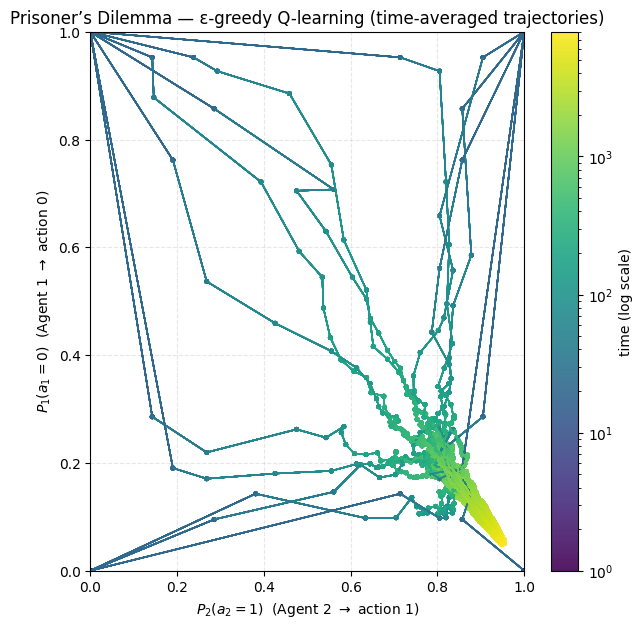
\includegraphics[width=\linewidth]{figures/task-2/learning/pd_egreedy.png}
        \caption*{(a) $\epsilon$-greedy Q-learning}
    \end{minipage}
    \hfill
    \begin{minipage}{0.32\textwidth}
        \centering
        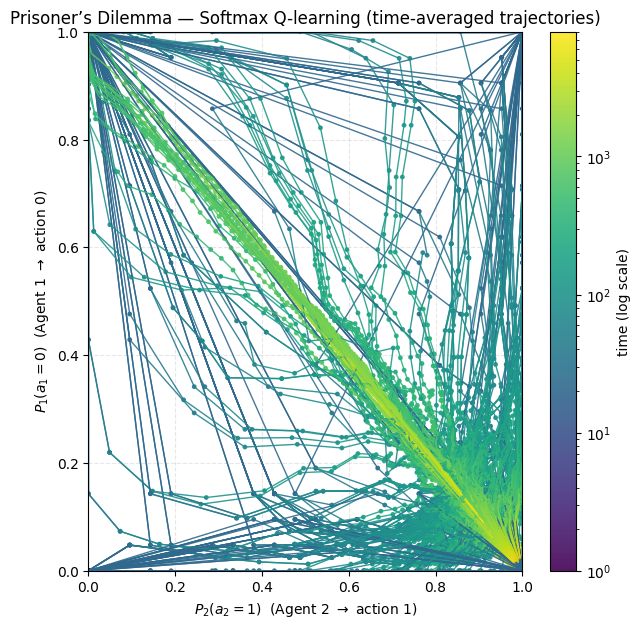
\includegraphics[width=\linewidth]{figures/task-2/learning/pd_boltz.png}
        \caption*{(b) Boltzmann Q-learning}
    \end{minipage}
    \hfill
    \begin{minipage}{0.32\textwidth}
        \centering
        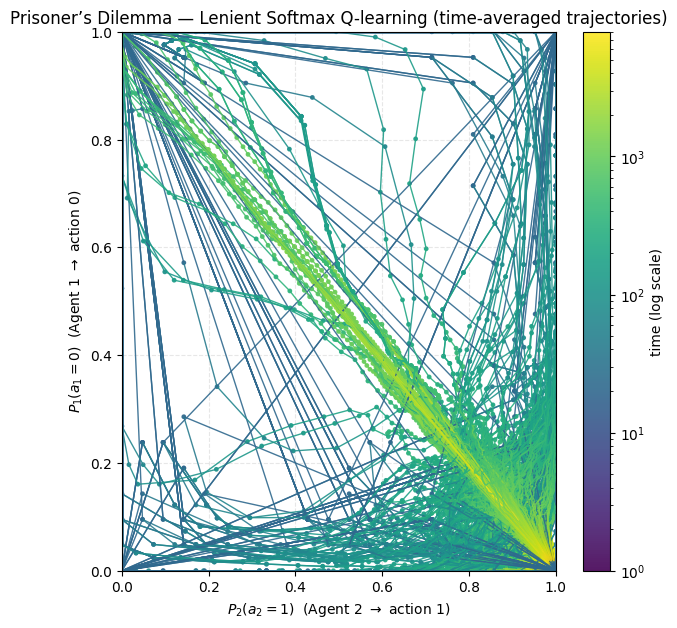
\includegraphics[width=\linewidth]{figures/task-2/learning/pd_lenient.png}
        \caption*{(c) Lenient Boltzmann Q-learning}
    \end{minipage}
    \caption{Empirical learning trajectories for the Prisoner's Dilemma using (a) $\epsilon$-greedy Q-learning, (b) Boltzmann Q-learning, and (c) Lenient Boltzmann Q-learning.}
\end{figure}



\subsection{Analitical analysis of the learning dynamics using replicator equations}
The learning dynamics of the algorithms are analyzed using replicator equations, which model how the proportion of strategies in a population change over time based on their relative payoffs. The replicator equations are visualized as vector fields over the strategy simplex, with arrows indicating the direction and magnitude of change in strategy proportions. The replicator dynamics of each game are plotted for Boltzmann Q-learning and Lenient Boltzmann Q-learning. The derivation of the equations and the implementation are in an appended notebook for clarity and reproducibility.

\begin{figure}
    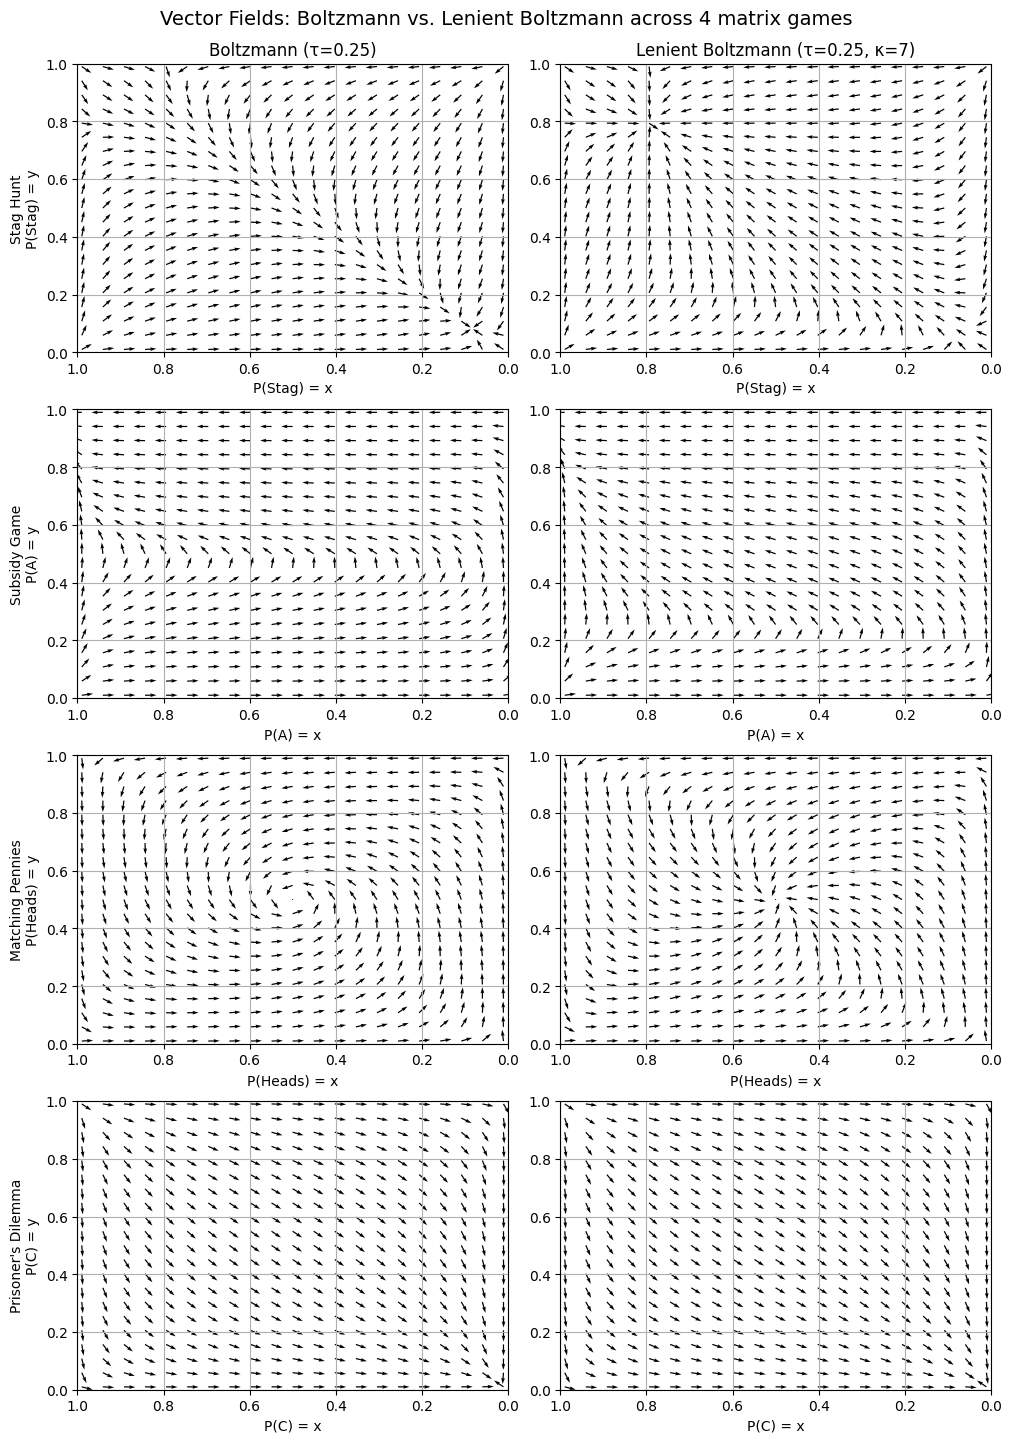
\includegraphics[width=\linewidth]{figures/task-2/replicator_dynamics.png}
\end{figure}

The learning behavior observed in the empirical trajectories match well with the predictions made by the replicator equations, confirming the validity of the analytical approach. The only inconsistency is that the replicator dynamics predict that Lenient Boltzmann Q-learning should be able to learn to cooperate in the Stag Hunt, while the empirical results show that it fails to do so. This discrepancy could be due to the specific parameters used in the learning algorithms, such as the learning rate, exploration rate, and leniency factor. Further tuning of these parameters might help align the empirical results with the theoretical predictions.


\section{Task 3: Single Archer Reinforcement Learning}

In this task a single archer agent (\texttt{archer\_0}) learns to play the
\emph{Knights Archers Zombies} (KAZ) environment, implemented in the
PettingZoo multi-agent reinforcement learning library \cite{pettingzoo2020}.
The reinforcement learning framework Ray RLlib \cite{liang2018rllib} is used
to implement and train the agent.

Following the classical foundations of reinforcement learning
\cite{sutton2018reinforcement}, we investigate two families of algorithms:
value-based methods (Deep Q-Networks, DQN \cite{mnih2015human}) and
policy-gradient methods (Proximal Policy Optimization, PPO
\cite{schulman2017proximal}). Both algorithms are first established as
minimal, controlled baselines, and then incrementally enhanced with canonical
improvements documented in the literature. 

A central difficulty in reinforcement learning research is understanding why a
given agent succeeds or fails. To address this, we adopt strict evaluation
protocols following Machado et al. \cite{machado2018revisiting}, including
the use of sticky actions to prevent brittle open-loop policies, disjoint
training and evaluation seed sets, multi-seed evaluation, and fixed
environment-interaction budgets. All experiments are run with a fixed seed per
configuration, each evaluated on $K=20$ episodes at regular checkpoints,
reporting mean returns. Performance is compared using
metrics such as final average return, area under the learning curve (AUC).

\subsection{Neural Network Size}
A crucial parameter in Deep learning is the size of the model. KAZ is a complicated game with subtle shooting mechanics combined with overal strategy and movement. The amount of features in the observation are however limited. Two hidden layers suffice to learn the features of vectorized observations like in our KAZ setup. The with of the hidden layers then decides the complexity of the model. A wide neural network will have a higher representational capacity and can make the learning more stable or smooth, yet it will be expensive to train and could be prone to overfitting, although the variation in the learning episodes will likely make it so that this is not a problem. A model that is too small will fail to understand the complex mechanics of targeting and shooting zombies and would fall back to cheap repetitive strategies, like failing to shoot at the lowest zombie. An experiment with an appropriate simple but effective learning algorithm compares three neural network sizes. (64,64) vs (128,128) vs (256,256) vs (512,512).

\subsubsection{Results}
The small neural network seems to be able to represent a sufficently sophisticated strategy. It learned to aim and shoot within less environment steps then the more complicated models. The more complicated models seem to learn either really slowly or fail to generalize. For KAZ two hidden layers with width 64 is the best approximator.

\subsection{Feature Engineering}
Feature engineering refers to the process of transforming raw observations into
more informative inputs that make learning easier for the agent. In reinforcement
learning, compact and well-designed observations can significantly reduce sample
complexity and improve generalization. For example, reducing the observation space
to only essential features often leads to more stable learning compared to using
large, noisy state vectors \cite{rauber2017hindsight}. In the KAZ case, we hypothesize
that replacing redundant heading vectors with alignment error vectors provides a
more direct learning signal for aiming tasks.

\subsection{Reward Shaping}
Reward shaping is the practice of modifying the environment's reward signal to
make it more informative and easier for the agent to learn from, while ideally
not changing the optimal policy \cite{ng1999policy}. In sparse-reward environments
such as KAZ, reward shaping can provide intermediate feedback that guides learning
towards useful behaviors. A particularly relevant example is survival-based reward
shaping: giving the agent a small positive reward for every timestep it remains
alive. This can encourage the agent to adopt evasive and strategic movement
patterns, rather than relying solely on killing zombies for reward.


\subsection{PPO Learning}

Proximal Policy Optimization (PPO) \cite{schulman2017proximal} is a popular
policy-gradient method that strikes a balance between stability and simplicity.
It constrains policy updates through a clipped objective, preventing destructive
large updates that could destabilize training. PPO generally achieves higher
sample efficiency and stability compared to vanilla policy gradient methods,
while avoiding the complexity of trust-region approaches such as TRPO. Its
robustness and ease of implementation make it one of the default choices for
continuous and discrete control tasks.

A practical advantage is that PPO is directly supported in \texttt{Ray RLlib},
with highly optimized implementations and configuration options available in
the official documentation\footnote{\url{https://docs.ray.io/en/latest/rllib/rllib-algorithms.html}}.


\subsection{Incremental PPO Evolution}

Starting from a plain PPO baseline with a simple MLP policy network, we
systematically introduce enhancements motivated by prior work on stabilizing
policy-gradient methods \cite{arulkumaran2017deep}. The incremental path is:

\begin{enumerate}
    \item \textbf{BASE} minimal PPO (no entropy bonus, no KL control, no observation normalization).
    \item \textbf{P1}  add entropy regularization to improve exploration.
    \item \textbf{P2}  add KL divergence control to stabilize policy updates.
    \item \textbf{P3}  apply gradient-norm clipping to mitigate instability.
    \item \textbf{P4}  increase GAE $\lambda$ from 0.95 to 0.98 to improve long-horizon credit assignment.
\end{enumerate}

\subsection{DQN Learning}

Deep Q-Networks (DQN) \cite{mnih2015human} extend traditional Q-learning to
high-dimensional state spaces by using a neural network to approximate the
action-value function. DQN introduced key innovations such as the use of an
experience replay buffer to decorrelate samples and a target network to
stabilize bootstrapping updates. Compared to policy-gradient methods, DQN is
value-based and often more sample efficient in discrete action spaces. While
extensions such as Double-DQN, Dueling architectures, and Prioritized Replay
have become standard, even the plain DQN baseline provides a strong foundation
for discrete-control tasks. 

Similar to PPO, DQN is straightforward to implement in \texttt{Ray RLlib},
which offers modular agents, replay buffers, and policy definitions. The
reference implementation is available in the official RLlib algorithms
documentation\footnote{\url{https://docs.ray.io/en/latest/rllib/rllib-algorithms.html}}.
\subsection{Incremental DQN Evolution}

A similar stepwise methodology is applied to DQN, starting from a minimal
baseline and progressively enabling improvements well-documented in the
literature \cite{mnih2015human, vanhasselt2016double, wang2016dueling,
schaul2015prioritized, bellemare2017distributional}:

\begin{enumerate}
    \item \textbf{BASE}  plain DQN (uniform replay, $n$-step=1, no Double, no Dueling).
    \item \textbf{D1}  increase to $n$-step returns ($n=3$).
    \item \textbf{D2}  enable Double-DQN to reduce overestimation bias.
    \item \textbf{D3}  add Prioritized Experience Replay (PER).
    \item \textbf{D4}  introduce Distributional DQN (C51).
\end{enumerate}

\subsubsection{Results}
All models were implemented and verified. Sadly, due to time constraints only partial runs were done and no proper experiments could be run to their conclusion. Informally this is what the test runs showed. The base implementation did learn how to properly shoot and play the game. Compared to PPO learning, it needed considerably more environment steps to reach the same level. In general the DQN models also seemed to benefit from using bigger neural networks. Introducing $n$-step in the D1 model was beneficial. Enabling Double-DQN made the learner faster to learn and smoother. Adding a prioritized Replay buffer seemed to kill the ability of the model to learn. This is strange and should be investigated properly. Introducing a distributional DQN improved the learner, but only slightly.

\subsection{LSTM Networks}

Long Short-Term Memory (LSTM) networks \cite{hochreiter1997long} are a
specialized type of recurrent neural network (RNN) designed to capture
long-range temporal dependencies in sequential data. Unlike simple RNNs, LSTMs
mitigate the vanishing and exploding gradient problems by introducing a gating
mechanism that controls the flow of
information. This allows LSTMs to retain relevant information over extended
time horizons, making them particularly effective for partially observable
environments or tasks where temporal context is essential.

In reinforcement learning, LSTMs are often used to augment policy or value
networks, enabling agents to integrate information across multiple timesteps
rather than relying solely on the current observation. This is especially
useful in settings with incomplete or noisy observations.

As with PPO and DQN, LSTM-based models are directly supported in
\texttt{Ray RLlib}, which provides recurrent policy templates and utilities for
sequence batching and hidden state management. Reference implementations are
documented in the RLlib algorithms guide\footnote{\url{https://docs.ray.io/en/latest/rllib/rllib-algorithms.html}}.

Implementations of a RRN in using both PPO and DQN are part of the source github. Due to time constraints, only informal results could be retrieved. The models did exhibit more deliberate strategy. The archer would occasionally move to catch a zombie that was near to the border. For both the DQN implementation and PPO implementation, it took much longer to train. Getting the parameters right was also more tricky. For the KAZ game in single player mode, I think it might be better to stick with simple models. 

\subsection{Conclusion}
Our experimentation tells us a couple things. KAZ is a complex games which can be learned using deep learning. When using vectorized observations a small neural network suffices to learn the game. Ray RLlib has readily available implementations for both DQN learning algorithms and PPO algorithms. For KAZ, PPO learning seems to outperform DQN learning. Reward shaping can be used to incentivise an agent to learn quicker by stimulating the actual desired behavior. Limiting the observation space is a good idea and helps simpler models to learn faster. Adding angular offsets to an aiming task makes learning easier. 

LSTM models are interesting, but harder to setup and more expensive to train. For KAZ the complexity might outweight the benefit.

\bibliographystyle{IEEEtran}  
\bibliography{references}


\end{document}
